\documentclass[draftclsnofoot,onecolumn,compsoc]{IEEEtran}

\usepackage[english]{babel}
\usepackage[utf8x]{inputenc}
\usepackage[T1]{fontenc}
\usepackage{tocloft}
\usepackage{geometry}
\usepackage{graphicx}
\usepackage{float}
\usepackage{hyperref}

\geometry{margin=0.75 in}

\addto\captionsenglish{\renewcommand{\contentsname}{TABLE OF CONTENTS}}

\begin{document}

\vfill

%---------------------------------------------%
%---------------- TITLE PAGE -----------------%
%---------------------------------------------%

\begin{titlepage}

\title{
  ~ \\ ~ \\ ~ \\ ~ \\ ~ \\
  Software Specification Design Document \\ \bigskip
  \large
  Group 61: iCreate - Generative Design in Virtual Reality \\
  April 23, 2018 - Winter Term}
    
\end{titlepage}

\author{Hannah Solorzano - Nabeel Shariff - Rhea Mae Edwards}

\maketitle

% As a general rule, do not put math, special symbols or citations 
% in the abstract or keywords.

\vfill

%---------------------------------------------%
%----------------- ABSTRACT ------------------%
%---------------------------------------------%

\begin{abstract}
\par \noindent
iCreate Generative Design in Virtual Reality is a software program that allows the user to create complex architectural structures using a series of spawned objects. As precision in movements and gestures are important, the UI has been designed in such a way that the user is unhindered and experiences a limited learning curve when using the software for the first time.
\end{abstract}

\newpage

%---------------------------------------------%
%--------------- PARTICIPANTS ----------------%
%---------------------------------------------%

\section*{PARTICIPANTS}
The ICreate - Generative Design in Virtual Reality senior software engineering project consists of the following team members:
\bigskip

\noindent\leavevmode\rlap{}\hfill{\textbf{Raffaele de Amicis,} \textit{Mentor}}\hfill\llap{}\par
\bigskip
\noindent\leavevmode\rlap{\textbf{Hannah Solorzano,} \textit{Software Developer}}\hfill{\textbf{Nabeel Shariff,} \textit{Software Developer}}\hfill\llap{\textbf{Rhea Mae Edwards,} \textit{Software Developer}}\par

\bigskip
\noindent
The following persons are associated with Intel Corporation in regards to Hardware, Software and Development Environments in relations to the project:
\bigskip

\noindent\leavevmode\rlap{}\hfill{\textbf{Mike Premi,} \textit{Co-Mentor}}\hfill\llap{}\par

\bigskip
\noindent
The following persons are guidance mentors as a part of the senior software engineering project course for the students:
\bigskip

\noindent\leavevmode\rlap{\textbf{Kevin McGrath,} \textit{Instructor}}\hfill{\textbf{Kirsten Winters,} \textit{Instructor}}\hfill\llap{\textbf{Behnam Saeedi,} \textit{Teaching Assistant}}\par

\newpage

%---------------------------------------------%
%------------- TABLE OF CONTENTS -------------%
%---------------------------------------------%

\tableofcontents 

\newpage

%---------------------------------------------%
%--------------- CONTRIBUTIONS ---------------%
%---------------------------------------------%

\section*{CONTRIBUTIONS} 
The members of the design team have contributed to the following sections as listed:
~ \\

\noindent
\textit{Hannah Solorzano:}
	\begin{itemize}
		\item Base formatting of \LaTeX  document
        \item Section 1: Introduction
        \item Section 2.0 / 2.1.2 / 2.1.4 / 3.1 / 3.6
        \item Section 2.1.1 / 3.2 (Co-authored with Nabeel)
        \item Section 4: Class Design
        \item Section 5: State Design
        \item Figures 1, 3, 4, 5, 6, 7, 8
	\end{itemize}

~ \\
\textit{Nabeel Shariff:}
	\begin{itemize}
		\item Section 2.1.1 /  3.2 (Co-authored with Hannah)
        \item Section 3.3/ 3.4 
        \item Figure 2
	\end{itemize}
    
~ \\
\textit{Rhea Mae Edwards:}
	\begin{itemize}
		\item Participants Section
        \item Section 3.5: Curves
	\end{itemize}

\newpage

%---------------------------------------------%
%-------- SECTION 1: INTRODUCTION ------------%
%---------------------------------------------%

\section{Introduction}

\subsection{Scope}
The software application described in this design document is to be utilized as a tool for the generative design of architectural structures. The goal of this software is not only to be used as a resource for the building of said structures, but also to be a tool for learning more about the limits of a standing structure.

\subsection{Purpose}
    The purpose of this Software Specification Document (SSD) is to provide a detailed description of the interface for the iCreate software. Included is the layout and functionality of the user interface.

\subsection{Intended Audience}
This document is intended for the stakeholders and architectural designers who intend to use this software. In addition, this SSD will be used as a reference for the stakeholders and Capstone professors in the case of a differing opinion in regards to the requirements of the design and performance.

\subsection{Definitions and Acronyms}
\begin{itemize}
\item \textbf{VR} -  An abbreviation of Virtual Reality which is described as, “the computer-generated simulation of a three-dimensional image or environment that can be interacted with in a seemingly real or physical way by a person using special electronic equipment, such as a helmet with a screen inside or gloves fitted with sensors.” [1]
\item \textbf{Virtual Space} - A 3D area in VR in which the user can maneuver around in and interact with objects.
\item \textbf{Generative Design} - A form finding process that can mimic nature’s evolutionary approach to design. [2]
\item \textbf{GUI} - The graphical user interface allows the user to interact with the program via buttons or other types of graphical icons.
\item \textbf{Primitive} - General 3D shape.
\item \textbf{Diegetic} - Interface that is included in the game world -- i.e., it can be seen and heard by the game characters.[3]
\end{itemize}

%---------------------------------------------%
%-- SECTION 2: SYSTEM ARCHITECTURE OVERVIEW --%
%---------------------------------------------%

\section{System Architecture Overview}

The iCreate software program is a developmental tool that can create architectural structure designs using the generative design process. As the user will be working with delicate structures, the GUI of the iCreate software must be laid out in a way that is intuitive, efficient, and neat.

\subsection{Design Viewpoints}

\subsubsection{Concerns of Design Stakeholders}
In regards to the developers, this software program should be simple and easily maintainable. The goal is to implement libraries and APIs that  provide the functionality in this program to reduce the complexity of the overall codebase. 

Users will be concerned about the overall look and feel of the software. The program’s interface must be polished, neat, and intuitive, allowing for a seamless and comfortable experience. The goal is for the user to be able to comfortably and successfully design projects with minimal interruptions.


\subsubsection{Context}
While developing the components of the iCreate software, the main consideration the developers had was the ease of use. As this program is meant for people with different types of technological backgrounds, the GUI must be easy to navigate.


\subsubsection{Interface}
Since iCreate’s user interface is meant for an intuitive experience, the developers have chosen to implement a design for the menu that is neat and robust at the same time, as well as comfortable for the user in terms of hand and eye strain.

\subsubsection{Structure}
Each of the components are separate objects which means that each primitive is able to have its own physics and settings. This makes manipulation of several primitives easier, and the learning curve smaller.

%---------------------------------------------%
%-------- SECTION 3: COMPONENT DESIGN --------%
%---------------------------------------------%

\section{Component Design}

\subsection{VR Environment}

The default scene for this software is an empty grey area. It was decided that an empty area would be best as it would reduce obstruction and distractions. Other scenes can have simple skyboxes with different floors to simulate a different scene. 

Locomotion will allow users to move around within the virtual environment, so the team will implement the keypad of one of the controllers to provide the user with a method of locomotion.

3D objects can be instantiated in the virtual environment by the users themselves. The user can spawn 3D objects by selecting from a menu of available primitives, and can also create multiple instances of that 3D object.


\subsection{User Interface}

The interface will need to functionally allow the user to spawn a 3D object, then modify it via either a controller or gesture input. Additionally, the user will be able to save to a library for later use or load their creations to create complex structures. Finally, the application will display a way to transform the 3D objects by allowing the user to scale or resize the object. 

\begin{figure}[h]
  \centering
    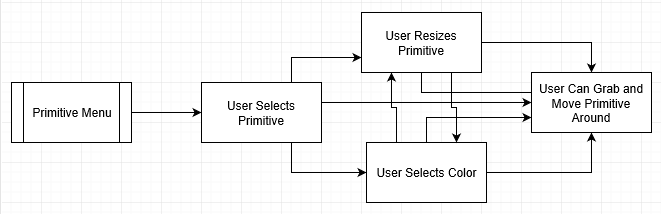
\includegraphics[width=0.8\textwidth]{new_menu}
    \caption{The flow of using the UI menu to spawn a shape. }
\end{figure}

The interface for iCreate will mostly be based on
Diegetic and spatial UI. Diegetic UI will be used for accessing tools and
options from a menu attached to the recessive hand’s controller, while for all other menus and uses, spatial UI will be used to relay relevant navigation
information to the user. The dominant hand will either be used to select
options from the menus presented to them, or draw within the virtual
Environment.  The general flow of spawning a shape is shown in Figure 1.
\\
\begin{figure}[H]
  \centering
    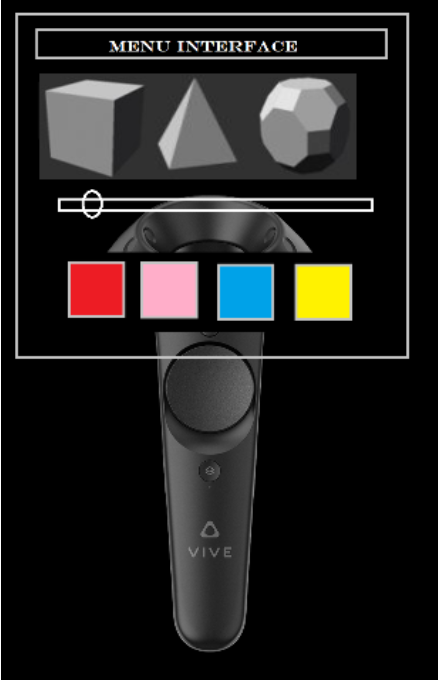
\includegraphics[width=0.5\textwidth]{menu}
    \caption{The UI menu that features the primitive and color options as well as the size slider. This menu will hover over the controller as a diegetic UI component}
\end{figure}

There are three sections to the menu which can be seen  in Figure 2. The first section has four primitives available to use: a square, circle, pyramid, and hexagon. The second part is a slider which can be used to adjust the size of the primitive spawned. Lastly, there are four color options for the primitives. As each primitive are separate objects, it is possible to have different combinations of sizes, colors, and shapes. 

\newpage

\subsection{Load and Save}
The save and load feature for iCreate can be realized through data serialization. To save the data of the scene, we will be using the FileStream and BinaryFormatter classes in Unity.

The FileStream class will be used to first create a save data file. Next, BinaryFormatter will be used to serialize the scene’s data into the save file. Once the data is serialized, FileStream can be used to close the file we were writing into.. 

Finally, to load the save file, BinaryFormatter can be used once again to deserialize the data from the save file and load the scene. The save and load features can be implemented via two buttons on the in game menu, one for saving and one for loading.

\subsection{Object Library}
The Object library will also utilize Unity’s serialization to save and load objects to and from a library of 3D objects created by the user. To save the object, BinaryFormatter can be used to save the attributes of the object, like position and rotation (x, y, z), material, etc, into a file or another GameObject. This file or GameObject will be the library. 

Finally, to load the saved object from the library into the game world, we can deserialize from the file or GameObject. The user can access and utilize the Object Library from within their in game menu.

\subsection{Curves}
\subsubsection{Drawing a Curve}
	The generation of a 3D within the program’s virtual environment, will be created with the user drawing a 3D curve in their space given. The program offer the user a variety of curves to choose from in order to start the generation of their curve, being a list containing the selections of a bezier curve, b-spline curve, ellipse curve, circle curve, hyperbola curve, and parabola curve. Each of these selections are characterized in the code as an equation with the possibility of an additional process in order to such curves depending on its type.

    After the user’s selection of a type of curve, the system will offer a base curve once the user selects a starting position within their given environment. Once the user selects the start of the curve, the program will adjust the size and trajectory of the curve itself based off the user’s physical movement of moving a controller around the environment from the starting position, generating the curve and sizing accordingly. The user’s movements of the controller will provide a variety of inputs for the system given the equation selected by the user earlier. After a button indication from the user, the generated curve will be set in place by the system, giving the finality of that curve within the environment.
\subsubsection{Circle Curves, Ellipse Curves, Hyperbola Curves, Parabola Curves}
	Circle curves, ellipse curves, hyperbola curves, and parabola curves have set alegbraic equations that can be written in code that represent these four types of code. The program will apply these equations along with the user’s curve drawing process explained above.
\subsubsection{Bezier Curves}
	For generating bezier curves within the program, the Handles.DrawBezier will be able to take in inputs such as the start position, end position, start tangent, and the end tangent of a bezier curve, which we are characteristics and inputs we are interested in creating in regards to the generation of such a curve. These inputs will be given by the user, from their selection of this curve type and then draw given these specifications within the environment. [4]
\subsubsection{B-Spline Curves}
	B-Spline Curves will inherit the same process when it comes to generating bezier curve within the program, but in addition with its slight difference of consisting multiple bezier curves generating a single b-spline curve. Due to a b-spline curve’s notable characteristic of smoothness with multiple peaks and lows, such a curve can be generated with multiple bezier curves in order to be physically represented.

\subsection{Transformation and Translation}
The transformation feature will be primarily used while the shape is being instantiated. During the creation, the user can choose to alter the size of the shape via sliders on the diegetic menu attached to the user’s controller. 

The translation feature allows the shapes to be maneuvered about the environment. The shapes are not influenced by gravity, so they will float in place. The user is then able to grab the shapes and move them around the environment at will. It was decided to not have the shapes under the effects of gravity to aide in the design process to prevent the shapes from rolling around.

%---------------------------------------------%
%-------- SECTION 4: CLASS DESIGN --------%
%---------------------------------------------%

\section{Class Design}
This section will describe the classes and methods available in iCreate and how they are related to each other. There are six main classes: Main Menu, Load Project, New Project, Project, Brick, and Algorithm as shown in Figure 3 below.
\\
\begin{figure}[H]
  \centering
    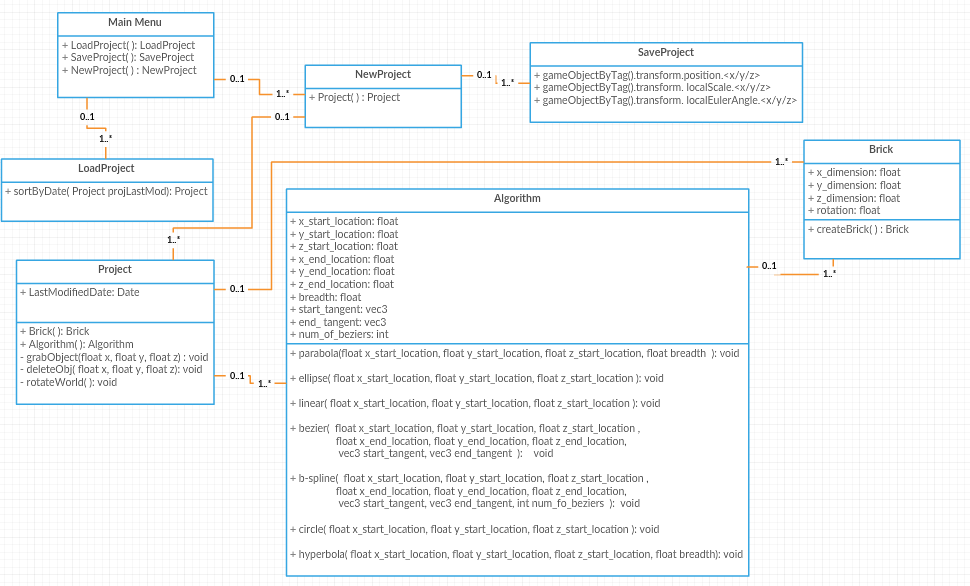
\includegraphics[width=0.9\textwidth]{Class_diagram}
    \caption{Class diagram that displays the methods available in iCreate, as well as the relationships between the different classes.}
\end{figure}

\newpage

\subsection{Main Menu}
The main menu is the first screen that the user encounters when opening the iCreate program and has three functionalities: Load Project, New Project, and Exit. While the \textit{Load( )} and \textit{NewProject( )} selections are passed to the LoadProject and NewProject classes respectively which lead the user into the VR environment. The \textit{Exit( )} selection exits the program entirely.

\subsubsection{Available Functions:}
\begin{itemize}
\item \textit{LoadProject( )} -\\
Calls the LoadProject class.
\item \textit{NewProject( )} -\\
Calls the NewProject class.
\item \textit{Exit( )} -\\
A public function that exits the program.
\end{itemize}

\subsection{Load Project}
When Load Project is selected from the main menu, a list of projects is  presented which are sorted by the projects' last date of modification using the \textit{sortByDate( )} function. This function cycles through each project and reads the Project's date variable \textit{lastModified}. After a project is selected, that project is then loaded into the VR environment to resume development.

This load feature works by reading from the saved file created by the SaveProject( ) function. It reads each of the location, rotation, and scale values and creates a block with those specifications using Unity's \textit{Instantiate( )} function.

\subsubsection{Available Functions:}
\begin{itemize}
\item \textit{sortByDate( Project projectLastMod )} -\\
A public function that is used by MainMenu's Load( ) to list the available projects. The parameter is a list of Projects, which will provide the last modification dates from calling \textit{Project.lastModifiedDate}. Returns a Project.
\item \textit{Project( )} -\\
Calls the Project class.
\end{itemize}

\subsection{New Project}
The New Project class enters into a new VR environment with no additional parameters or function calls.

\subsubsection{Available Functions:}
\begin{itemize}
\item \textit{Project( )} -\\
Calls the Project class.
\end{itemize}

\subsection{Save Project}
The Save Project class allows the current project to be saved by reading in the positions, rotation, and scale of each block and writing them to a file. As each block is being created, they are added to a block list. Present in this save function is a loop that cycles through every block in the list of blocks and reading the values of each block. These values will then be transformed into a string which will be written to a file in a data structure type format.

\subsubsection{Available Functions:}
\begin{itemize}
\item \textit{gameObjectByTag().transform.position.<x/y/z> } -\\
This function returns the x, y, and z coordinate location of a block.
\item \textit{gameObjectByTag().transform. localScale.<x/y/z> } -\\
This function returns the x, y, and z coordinates for the scale of a block.
\item \textit{gameObjectByTag().transform. localEulerAngle.<x/y/z>  } -\\
This function returns the x, y, and z coordinates for the angle of the block.
\end{itemize}

\subsection{Project}
The Project class is the VR environment where the user is able to design architectural structures. This class is related to the Brick and Algorithm class which enable the ability to spawn blocks in a specified pattern. The user is able to grab and delete blocks using the functions \textit{grabObj( )} and \textit{deleteObj( )}.The function \textit{rotateWorld( )} is used by the user to rotate the VR environment around for better viewing.

\subsubsection{Available Variables:}
\begin{itemize}
\item \textit{lastModifiedDate} - \\
A public variable that returns the date of the last modification to that Project. This variable is a Date.
\end{itemize}

\subsubsection{Available Functions:}
\begin{itemize}
\item \textit{grabObj(float x, float y, float z )} -\\
A private function that takes an x, y, z coordinate of the location of the object that is to be manipulated through the aid of a bounding box surrounding the head of the controller. Returns nothing.
\item \textit{deleteObj( )} - \\
A private function that takes an x, y, z coordinate of the location of the object that is to be deleted. Returns nothing.
\item \textit{rotateWorld( )} -\\
A private function that has no parameters. This function rotates the environment around the user. Returns nothing.
\end{itemize}

\subsection{Brick}
The brick class is used to instantiate the brick object, or primitive, and requires an x, y, and z dimension. The function \textit{createBrick( )}, takes the x, y, and z dimension parameters and spawns a brick with the specified size at the controllers' current location. 

\subsubsection{Available Variables:}
\begin{itemize}
\item \textit{x\_dimension} - \\
A public variable that specifies the x dimension of the brick. This variable is a float.
\item \textit{y\_dimension} - \\
A public variable that specifies the y dimension of the brick. This variable is a float.
\item \textit{z\_dimension} - \\
A public variable that specifies the z dimension of the brick. This variable is a float.
\end{itemize}

\subsubsection{Available Functions:}
\begin{itemize}
\item \textit{createBrick( float x, float y, float z )} -\\
A public function that takes three parameters which specify the size of the brick. Returns a Brick object.
\end{itemize}

\subsection{Algorithms}
The Algorithms class provides the user with the ability to spawn multiple Bricks along a calculated trajectory. This class offers four path types: Linear, Bezier, Ellipse, and Parabola. Each path function requires an x, y, and z coordinate to specify the starting location of the trajectory. 

\subsubsection{Available Variables:}
\begin{itemize}
\item \textbf{\textit{x\_start\_loc}} - \\
A public variable that specifies the x position of the starting point. This variable is a float.
\item  \textbf{\textit{y\_start\_loc}} - \\
A public variable that specifies the y position of the starting point. This variable is a float.
\item  \textbf{\textit{z\_start\_loc}} - \\
A public variable that specifies the z position of the starting point. This variable is a float.
\item  \textbf{\textit{x\_end\_loc}} - \\
A public variable that specifies the x position of the ending point of the given curve. This variable is a float.
\item  \textbf{\textit{y\_end\_loc}} - \\
A public variable that specifies the y position of the ending point of the given curve.. This variable is a float.
\item  \textbf{\textit{z\_end\_loc}} - \\
A public variable that specifies the z position of the ending point of the given curve. This variable is a float.
\item  \textbf{\textit{breadth}} - \\
A public variable that is calculated for the width of a trajectory based off the current angle of the controller and its given location.
\item  \textbf{\textit{start\_Tangent}} - \\
A public variable for the beginning tangent for a specified curve.
\item  \textbf{\textit{end\_Tangent}} - \\
A public variable for the beginning tangent for a specified curve.
\item \textbf{\textit{num\_of\_beziers}} - \\
A public variable that specifies the number of bezier curves to use when creating a B-spline trajectory.
\end{itemize}


\subsubsection{Available Functions:}
\begin{itemize}
\item \textbf{\textit{Parabola}}( float \textbf{x\_start\_loc} , float \textbf{y\_start\_loc}, float \textbf{z\_start\_loc},  vec3 \textbf{breadth} ) -\\
A public function that takes four parameters: three for the initial starting location of the trajectory, and one for the breadth of the curve. This function generates a parabolic curve using 30 control points that spread out a certain distance based off of the rotation of the controller - the higher degree of angle that the controller is in, the narrower the breadth of the curve is, and vise versa as seen in Figure 4. \\

%-						-----------------       %

\item \textbf{\textit{Ellipse}}( float \textbf{x\_start\_loc} , float \textbf{y\_start\_loc}, float \textbf{z\_start\_loc} ) -\\
A public function that takes three parameters which specify the beginning location of the ellipse trajectory. This function uses the click of the trigger button to begin a \textit{LineRenderer} component which initializes a circular line with a radius of 10 units. This circle's width can then be adjusted by dragging the controller while the trigger button is pressed. This method is illustrated in Figure 6. \\

%-						-----------------       %


\item \textbf{\textit{Linear}}( float \textbf{x\_start\_loc} , float \textbf{y\_start\_loc}, float \textbf{z\_start\_loc} ) -\\
A public function that takes three parameters - x, y, and z coordinate points for the beginning location. Once the beginning point is specified, the function generates a mesh cylinder of length 10 using the \textit{Mesh} component that represents the line. Calculations are done to change the center of rotation of the cylinder line from the center, to the origin point. This allows the line to be rotated around in a circle as seen in Figure 5.\\

%-						-----------------       %

\item \textbf{\textit{Bezier}}( float \textbf{x\_start\_loc}, float \textbf{y\_start\_loc}, float \textbf{z\_start\_loc},\\
\indent \hspace{10mm} float \textbf{x\_end\_loc}, float \textbf{y\_end\_loc}, float \textbf{z\_end\_loc}, \\
\indent \hspace{10mm}vec3 \textbf{start\_tangent}, vec3 \textbf{end\_tangent} ) -\\
A public function that takes 8 parameters which specify the beginning and ending location of the Bezier trajectory along with their respective tangent vectors. This function uses the \textit{DrawBezier} method of the \textit{Handles} class that is built into Unity. The \textit{DrawBezier} method requires the three coordinates of both the starting and ending locations, the two tangent vectors associated with each location, the color of the bezier, the texture, and the width. While the starting and ending locations will be passed into the function along with the tangent vectors, the color of the bezier curve will be set to red, the texture set to null, and the width set to the handle size * 0.1. This method is illustrated in Figure 7. \\

%-						-----------------       %

\item \textbf{\textit{B-Spline}}( float \textbf{x\_start\_loc}, float \textbf{y\_start\_loc}, float \textbf{z\_start\_loc},\\
\indent \hspace{14mm} float \textbf{x\_end\_loc}, float \textbf{y\_end\_loc}, float \textbf{z\_end\_loc}, \\
\indent \hspace{14mm}vec3 \textbf{start\_tangent}, vec3 \textbf{end\_tangent}, int \textbf{num\_of\_beziers} ) -\\
This function utilizes the Bezier function to create a Bezier Spline (B-spline) trajectory. The function takes 9 parameters: 2 for the beginning of the bezier, 2 for the ending location of the bezier, 2 tangent vectors which act as the middle two control points, and the last parameter is the number of bezier curves used to create the B-spline curve. Using the same functional methods as the Bezier function, this function cycles through creating and connecting the specified number of bezier curves to form the B-spline trajectory. This method is illustrated in Figure 7. \\


%-						-----------------       %

\item \textbf{\textit{Circle}}( float \textbf{x\_start\_loc} , float \textbf{y\_start\_loc}, float \textbf{z\_start\_loc} ) -\\
A public function that takes three parameters which specify the beginning location of the ellipse trajectory. This function is similar to the Ellipse function which uses the click of the trigger button to begin a \textit{LineRenderer} component that initializes a circular line with a radius of 10 units. This method is illustrated in Figure 6. \\

%-						-----------------       %

\newpage

\item \textbf{\textit{Hyperbola}}( float \textbf{x\_start\_loc} , float \textbf{y\_start\_loc}, float \textbf{z\_start\_loc}, vec3 \textbf{breadth} ) -\\
A public function that takes three parameters which specify the beginning location of the ellipse trajectory. This function utilizes the Parabola function to create an initial parabolic curve. Once this curve has been instantiated, the function uses the current angle of the controller to tilt the hyperbolic curve. This method is illustrated in Figure 4. \\
\end{itemize}

%-						-----------------       %

\begin{figure}[H]
  \centering
    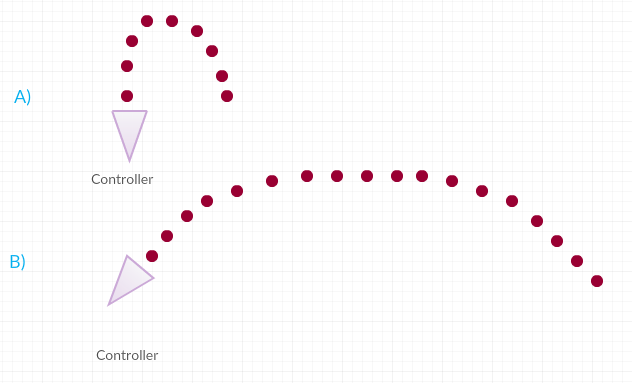
\includegraphics[width=0.8\textwidth]{parabola}
    \caption{The width of the parabola created using the Parabola( ) function is determined by the angle of the controller as seen by the difference between A and B. The dots represent the units that make up the trajectory. In the program, there will be 30 units per parabola. This method is also used for the Hyperbola( ) function, though the difference is that the tilting the controller on it's side will cause the trajectory to be drawn on it's side as well. }
\end{figure}


\begin{figure}[H]
  \centering
    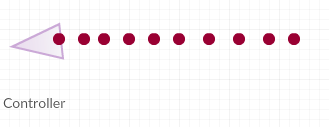
\includegraphics[width=0.8\textwidth]{linear}
    \caption{The Linear( ) function uses the head of the controller as the starting location for the linear trajectory. The trajectory is 10 units long. }
\end{figure}

\begin{figure}[H]
  \centering
    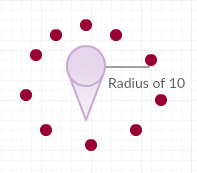
\includegraphics[width=0.6\textwidth]{ellipse}
    \caption{For both the Ellipse( ) and Circle( ) functions, the controller is set to the middle of the circle/ellipse while the trajectory is drawn around it. The circle/ellipse has a radius of 10, and depending on if it is a circle or ellipse being generated, the sides of the trajectory can be brought in to create a narrower path. }
\end{figure}

\begin{figure}[H]
  \centering
    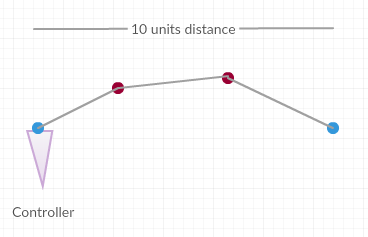
\includegraphics[width=0.7\textwidth]{bezier}
    \caption{The Bezier( ) function uses the head of the controller as the first point, and creates the end point 10 units away. In between, the two control points are created. The B-Spline( ) function uses the Bezier( ) function multiple times to create the B-spline path. For each call to the Bezier( ) function that is made, the ending point becomes the new starting point, with a new ending point being created 10 units away. }
\end{figure}
\newpage

\newpage

%---------------------------------------------%
%-------- SECTION 5: STATE DESIGN --------%
%---------------------------------------------%

\section{State Design}
This section describes the flow from state to state, as well as each choice presented at each step. Figure 8 shows the relationships between the various states and the destinations with the solid blue circle being the starting point, the squares representing the states, the orange circles representing the choices, and the blue dot with a ring being the end.
\begin{figure}[H]
  \centering
    %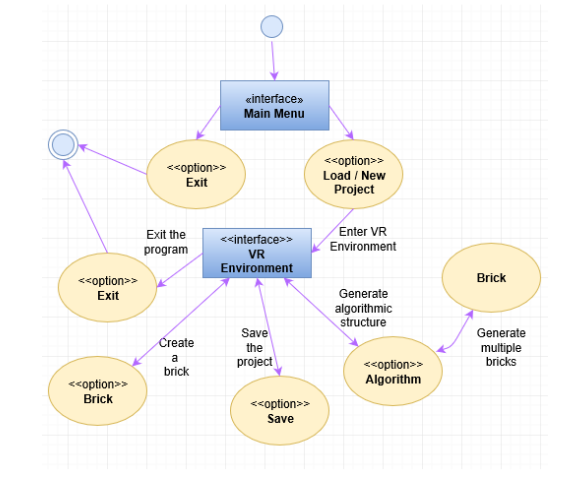
\includegraphics[width=0.8\textwidth]{State_Diagram}
    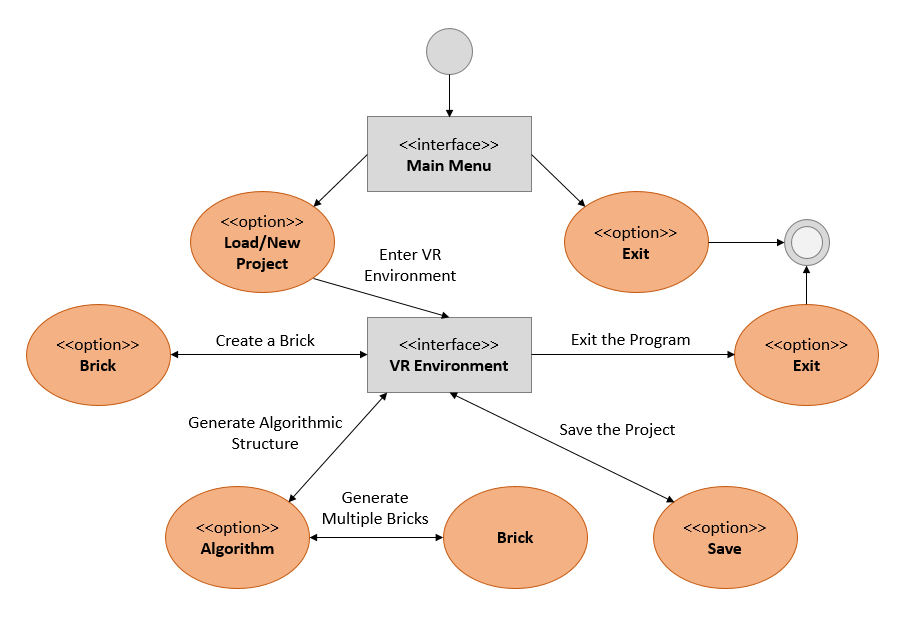
\includegraphics[width=0.8\textwidth]{state_diagram}
    \caption{State diagram that discloses the various states and choices the user is presented with when using the iCreate program. }
\end{figure}

When beginning the program, the user is shown the Menu which has several options that have two different destinations. If the user selects the Exit, then they will leave the program entirely, whereas if the individual selects either Load or New Project, they will enter into the main VR Environment. From this state, the user has four options: Create a brick, Save the current project, use an Algorithm, and Exit. The Brick, Save, and Algorithm choices will redirect the user back to the VR Environment state after finishing the choices' requested task. The Algorithm option will call on the Brick method multiple times to spawn the required number of bricks.The Exit choice will result in leaving the program. It is possible to leave the program without saving the current build.

\newpage
%---------------------------------------------------%
%--------------- LIST OF FIGURES-------------------%
%---------------------------------------------------%

\listoffigures

%---------------------------------------------%
%--------------- REFERENCES ------------------%
%---------------------------------------------%

\begin{thebibliography}{9}

\bibitem{first}
M. Webster (2018). 
\textit{Definition of Virtual Reality} 
. [Online]. Available: 
\\\url{https://www.merriam-webster.com/dictionary/virtual\%20reality}
\\

\bibitem{second}
AutoDesk (2018). 
\textit{What is Generative Design} 
. [Online]. Available: 
\\\url{https://www.autodesk.com/solutions/generative-design}
\\

\bibitem{third}
Gamasutra (2018). 
\textit{Game UI Discoveries: What Gamers Want} 
. [Online]. Available: 
\\\url{https://www.gamasutra.com/view/feature/4286/game_ui_discoveries_what_players_.php?print=1}
\\

\bibitem{fourth}
Unity Technologies (2018). 
\textit{Handles.DrawBezier} 
. [Online]. Available: 
\\\url{https://docs.unity3d.com/ScriptReference/Handles.DrawBezier.html}
\\

\end{thebibliography}
\end{document}


